\section{Unweighted transverse spherocity \SOPT}
\label{Sec:SOPT}

In this analysis, the unweighted transverse spherocity \SOPT is used to
quantify the topology in the azimuthal plane. It is calculated as
\begin{equation}\label{Eq:SOPT}
\centering
    \SOPT = \frac{\pi^2}{4} \min_{\hat{n}} \left(\frac{\Sigma_i
      |\hat{p_{\textrm{T},i}} \times \hat{n}|}{N_{\textrm{trks}}}  \right)^{2}.
\end{equation}
The sum is calculated over all charged particles with $\pt > \gevc{0.15}$, where $\hat{p_{\textrm{T}}}$ represents the transverse momentum unit vector, $N_{\textrm{trks}}$ is the number of charged particles in a given event and $\hat{n}$ is the unit vector that minimizes \SOPT. 

Loose selection criteria were chosen for primary tracks to ensure a high efficiency and uniform azimuthal acceptance over the full TPC volume. At least 50 or more measured clusters are required for a track in the TPC. Furthermore, the TPC tracks must be matched to hits in the ITS, but, to ensure homogeneous azimuthal acceptance, the tracks are not explicitly required to have hits in the SPD. These requirements improve the tracking precision, and reject tracks from out-of-bunch pile-up. Finally, selections of distance of closest approach (DCA) along the beam axis ($|\rm DCA_{\it{z}}|<3.2 $ cm), and in the xy-plane ($|\rm DCA_{\it{xy}}|<2.4 $ cm) are applied, ensuring that the reconstructed TPC track points to the primary vertex.

Unlike the traditional transverse spherocity estimator discussed in~\cite{ALICE:2019dfi}, the transverse momentum ($\pt$) of each track in this article is normalized to 1 ($\pt = 1$) when measuring the \SOPT. This modification was required to have similar sensitivity between neutral and charged particles. Otherwise, there would be significant differences between the production of neutral and charged kaons in jet-like events. This can be understood considering that for the traditional spherocity, a single high-\pt track will have a large weight in the spherocity calculation, which can occur for a charged kaon but never for a neutral kaon. By assigning the same weight to all measured primary charged tracks, one reduces the possible charged-vs-neutral biases.

However, this also means that results obtained with the two different spherocity estimators (traditional and unweighted) can only be qualitatively compared. Furthermore, as \SOPT is independent of the \pt of the particles, it requires a substantial amount of particles to be a good measure of the event topology. For this reason, the number of charged tracks is required to be greater or equal to 10 for events included in this analysis, which limits the applicability of the unweighted spherocity estimator to only apply for high-multiplicity pp collisions, where the average \dndeta is greater than 10.

The values of \SOPT will, by construction, lie between 0 and 1. Having events with $\SOPT \approx 0$ imply that $|\hat{p_{\textrm{T}}} \times \hat{n}| \approx 0$ for all tracks, which indicates that all tracks are parallel in the azimuthal plane, suggesting that the event is dominated by a single back-to-back dijet. Events where \SOPT $\rightarrow$ 1 imply that all particles are uniformly distributed azimuthally, suggesting the absence of a preferred direction. Note that part of the isotropy of the event can be affected by anisotropic flow~\cite{Ref:Flow1}. The unfolded \SOPT distributions are presented in Fig.~\ref{Fig:SO}, along with model predictions, for the three different multiplicity selections used in this article. Particle candidates that enter into the \SOPT calculation for the model predictions are required to meet the ALICE definition of a primary charged particle~\cite{alice_primary}.  The correction of the \SOPT distributions is based on the Bayesian unfolding technique~\cite{DAgostini:1994fjx}. The same unfolding method used in previous ALICE publications~\cite{ALICE:2023yuk} is applied here.

It is crucial to emphasize that, unlike the distributions presented in Fig.~\ref{Fig:SO}, the individual particle \pt-spectra are not corrected with Bayesian unfolding.
A key aspect of the analysis presented in this article is the capability to compare the measured results with MC generator predictions. Extensive studies were performed to understand and mitigate any experimental biases due to the \SOPT selection. The experimental bias is evaluated by generating PYTHIA 8~\footnote{The fully simulated PYTHIA events are the same used to obtain the tracking efficiency correction discussed in Sec.~\ref{Sec:Details}. We refer to this section for technical details on the simulation.} events, that are propagated through a full ALICE simulation of the experimental apparatus. The \SOPT definition has been constructed to require that the generated events agree with the reconstructed simulated events, where the \pt spectra have been corrected for the minimum bias reconstruction efficiency\footnote{Secondary particles were rejected using MC information.}. This ensures that the measured and generated results are directly comparable, where the measured results do not require further unfolding. This is achieved by adopting the following criteria, which minimizes the experimental uncertainty and makes \SOPT a robust and model-independent observable:


\begin{itemize}
    \item \textbf{\SOPT selection in quantiles.}\\
    One major source of experimental bias is the smearing of the measured \SOPT distribution by detector effects. It was verified through MC studies that one can minimize the effect of the smearing by measuring \SOPT in quantiles, similar to how multiplicity classes are defined in ALICE~\cite{ALICE:2019dfi}. The stability of the quantiles is due to the fact that spherocity distribution does not have large gradients. A robust model-to-data comparison is achieved by calculating the model comparison in measured percentiles, rather than for the numerical \SOPT ranges we report in this article.
\end{itemize}

\begin{itemize}
    \item \textbf{Exclusion of neutral decay modes for resonance particles}\\
    The decay daughters of both \PHI and \KSTAR meet the standard ALICE definition of primary particles~\cite{alice_primary}, subsequently leading to the resonance daughters entering the measurement of \SOPT for a given event. These daughters will contribute to the multiplicity estimate if measured at midrapidity, and as both the \PHI and \KSTAR resonances have charged and neutral decay modes, the branching ratio for the charged decay mode will artificially inflate in high-multiplicity events. This bias can be completely avoided by only including (and correcting for) the following charged decay modes for resonance particles in the resulting spectra: \PHI $\rightarrow$ $K^+K^-$ and \KSTAR $\rightarrow$ K\PI. 
\end{itemize}

\begin{itemize}
    \item \textbf{Contamination of secondary particles}\\
    There is an effect that comes from the loose selection criteria for primary tracks used in this analysis. The loose DCA selections, which are there to maintain a full azimuthal acceptance, consequently lead to some decay daughters from $V^0$s and cascades to be incorrectly reconstructed as primary particles. To minimize the experimental bias from this effect, we include the primary \LA, \KOs, and \XI directly into the calculation of \SOPT for the generated MC predictions. The inclusion of these particles at the generator level makes the results presented in this article directly comparable to model predictions. 
\end{itemize}

 Note that the \SOPT distribution is the same across all presented particle species in this article. The implementation of these corrections reduce the experimental bias to a few percent, presented in Table~\ref{Tab:S0bias}, which lists the remaining fractional systematic uncertainties due to the \SOPT selection. The only exception is for low \pt \LA(\AL) and \KOs, where we do not present results for $\pt < \gevc{1}$. Our understanding is that for these very low \pt tracks, the azimuthal angles of the decay daughters that enter the \SOPT measurement are too different from their mother to give a precise result. Charged pions, kaons and (anti)protons are the most abundant particles, as well as the particles that enter directly into the \SOPT measurement, ensuring that these particle species are more robust against experimental biases. 

\begin{table}[h!]
\centering
\caption{The fractional systematic uncertainties used to estimate the experimental bias introduced when triggering on \SOPT. These uncertainties are a conservative estimate, obtained from the narrow \SOPT selections utilized in this analysis. The uncertainties are \pt-independent, and are applied to both jet-like and isotropic event selections, unless otherwise specified.}\label{Tab:S0bias}

\begin{tabular}{|l|cccccc|}
\multicolumn{1}{r}{\parbox[b][1.4em]{2em}{} } & \PI & K & p & $\mathrm{\phi}$ and $\mathrm{K}^{*}$ & \KOs and \LA & \multicolumn{1}{c}{$\Xi$} \\ \hline
\parbox[b][1.2em]{2em}{} &  &  &  &  & \pt$>1$ \GeVc &   \\
\SOPT \pt spectra & 0\% & 0\% & 0\% & 3\% & Isotropic: 1\% & 3\%  \\
  &  &  &  &  & jet-like: 4\% &   \\ \hline
\parbox[b][1.2em]{2em}{} &  &  &  &  & \pt$>1$ \GeVc &   \\
\SOPT h/\PI ratio & N/A & 0\% & 0\% & 3\% & Isotropic: 1\% & 3\%  \\
  &  &  &  &  & jet-like: 4\% &   \\ \hline  


\end{tabular}
\end{table}

The unfolded numerical ranges for the selected multiplicity and \SOPT quantiles are listed in
Table~\ref{Tab:SOPT}. The roman numerals represent the multiplicity labels for these percentiles reported in earlier ALICE publications~\cite{ALICE:2019dfi,ALICE:2023yuk}. It is important to stress that the \SOPT selections for the model comparisons presented throughout this article are done on their corresponding \SOPT quantiles, not the numerical quantities listed in Table~\ref{Tab:SOPT}.

\begin{table}[h!]
\centering
\caption{Values corresponding to the \SOPT ranges of different quantiles used for the event selections in this analysis, obtained from the corrected \SOPT distribution.}\label{Tab:SOPT}

\begin{tabular}{|cc|ccc|}
\hline
\multicolumn{2}{|r|}{\parbox[b][1.2em]{2em}{} Multiplicity:} & \tracklet I--III (0--10\%) & \tracklet I (0--1\%) & V0M I (0--1\%) \\ \hline
\multicolumn{5}{l}{\parbox[b][1.4em]{1em}{Jet$\text{-}$like}} \\ \hline
\multicolumn{2}{|l|}{\parbox[b][1.1em]{1em}{}\SOPT 0--1\%} & $<0.423$ & $<0.503$ & $<0.453$ \\
\multicolumn{2}{|l|}{\SOPT 0--5\%} & $<0.523$ & $<0.588$ & $<0.553$ \\
\multicolumn{2}{|l|}{\SOPT 0--10\%} & $<0.573$ & $<0.633$ & $<0.603$ \\
\multicolumn{2}{|l|}{\SOPT 0--20\%} & $<0.638$ & $<0.689$ & $<0.663$ \\
\hline
\multicolumn{5}{l}{\parbox[b][1.2em]{1em}{Isotropic}} \\ \hline
\multicolumn{2}{|l|}{\parbox[b][1.1em]{1em}{}\SOPT 80--100\%} & $>0.838$ & $>0.863$ & $>0.858$ \\
\multicolumn{2}{|l|}{\SOPT 90--100\%} & $>0.878$ & $>0.898$ & $>0.888$ \\
\multicolumn{2}{|l|}{\SOPT 95--100\%} & $>0.903$ & $>0.918$ & $>0.913$ \\
\multicolumn{2}{|l|}{\SOPT 99--100\%} & $>0.933$ & $>0.943$ & $>0.943$ \\ \hline
\end{tabular}
\end{table}


\begin{figure}[htbp!]
    \centering
    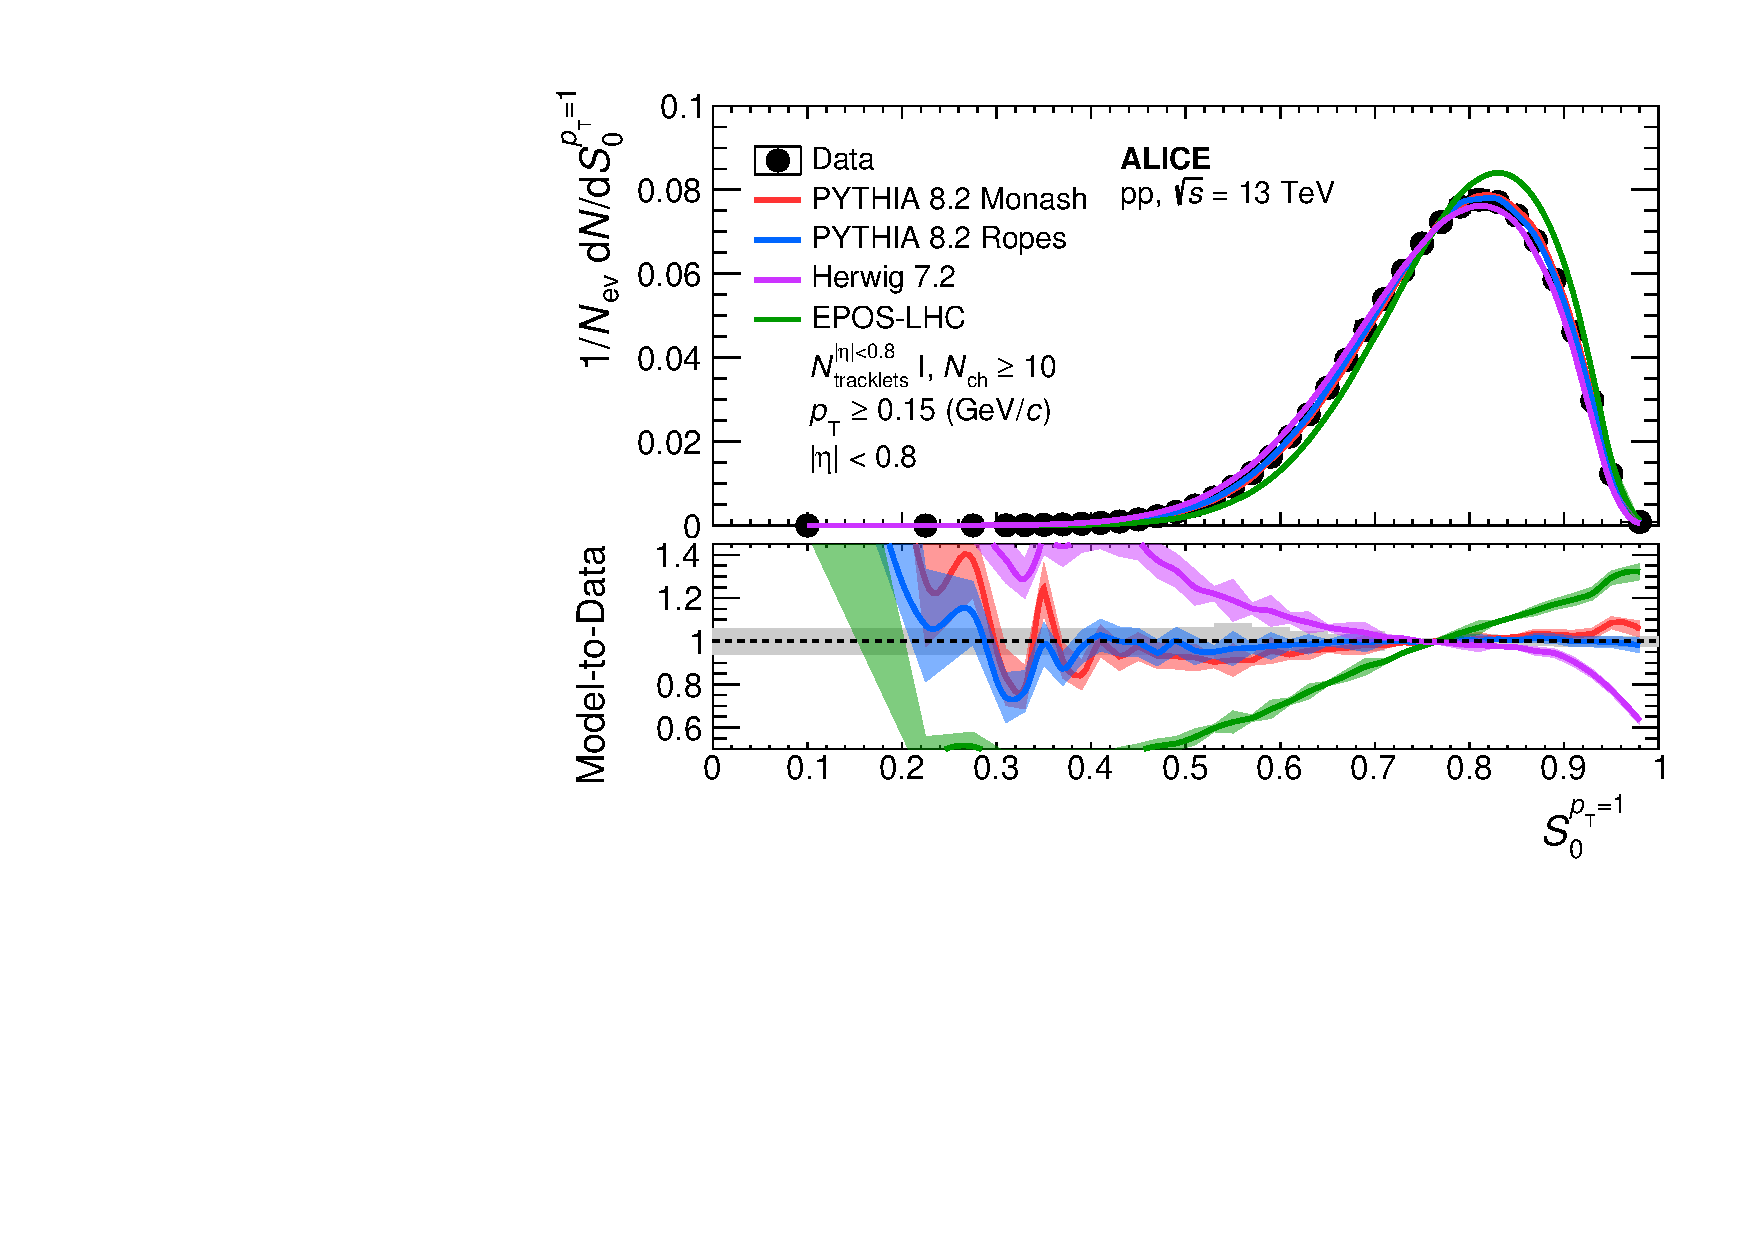
\includegraphics[scale=0.5]{figures/SO_Unfolded_cl1_Perc_I.pdf}
    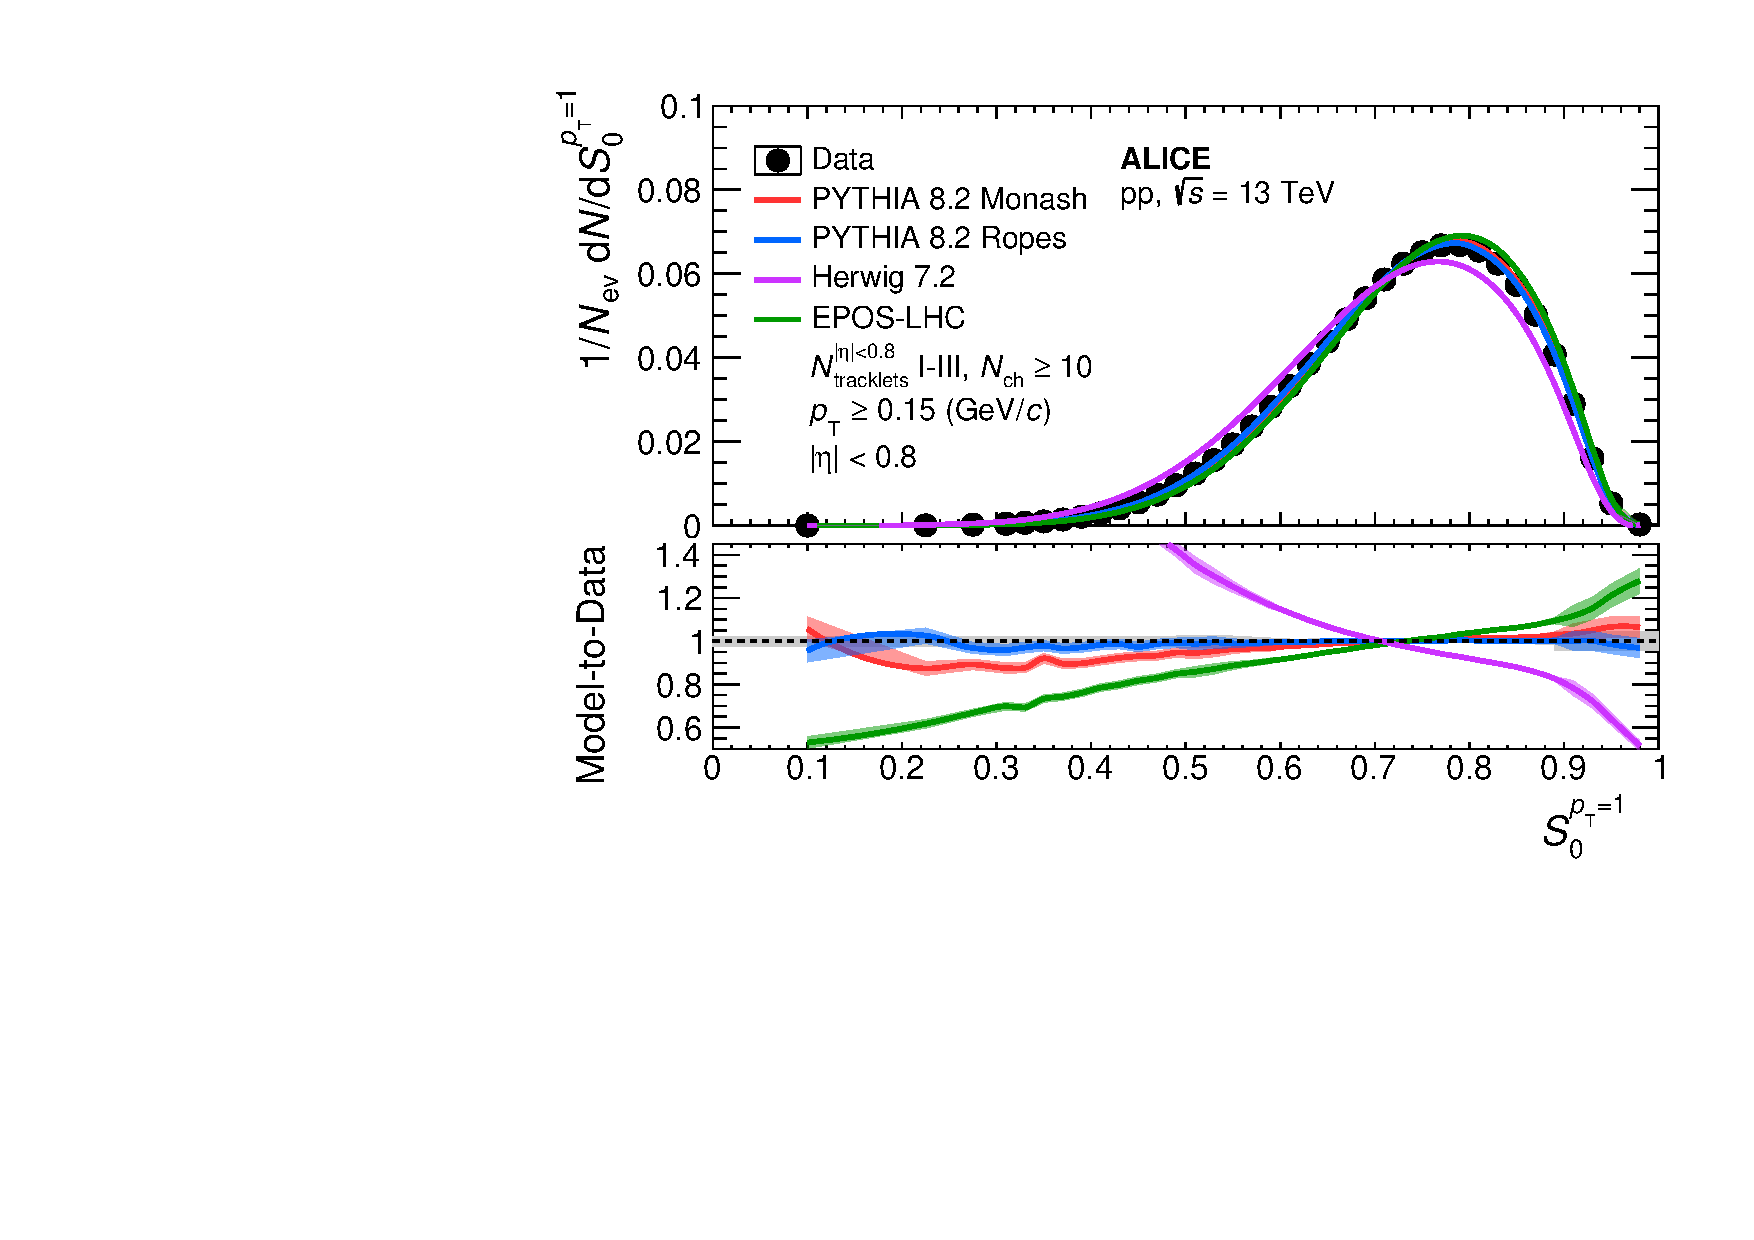
\includegraphics[scale=0.5]{figures/SO_Unfolded_cl1_Perc_III.pdf}
    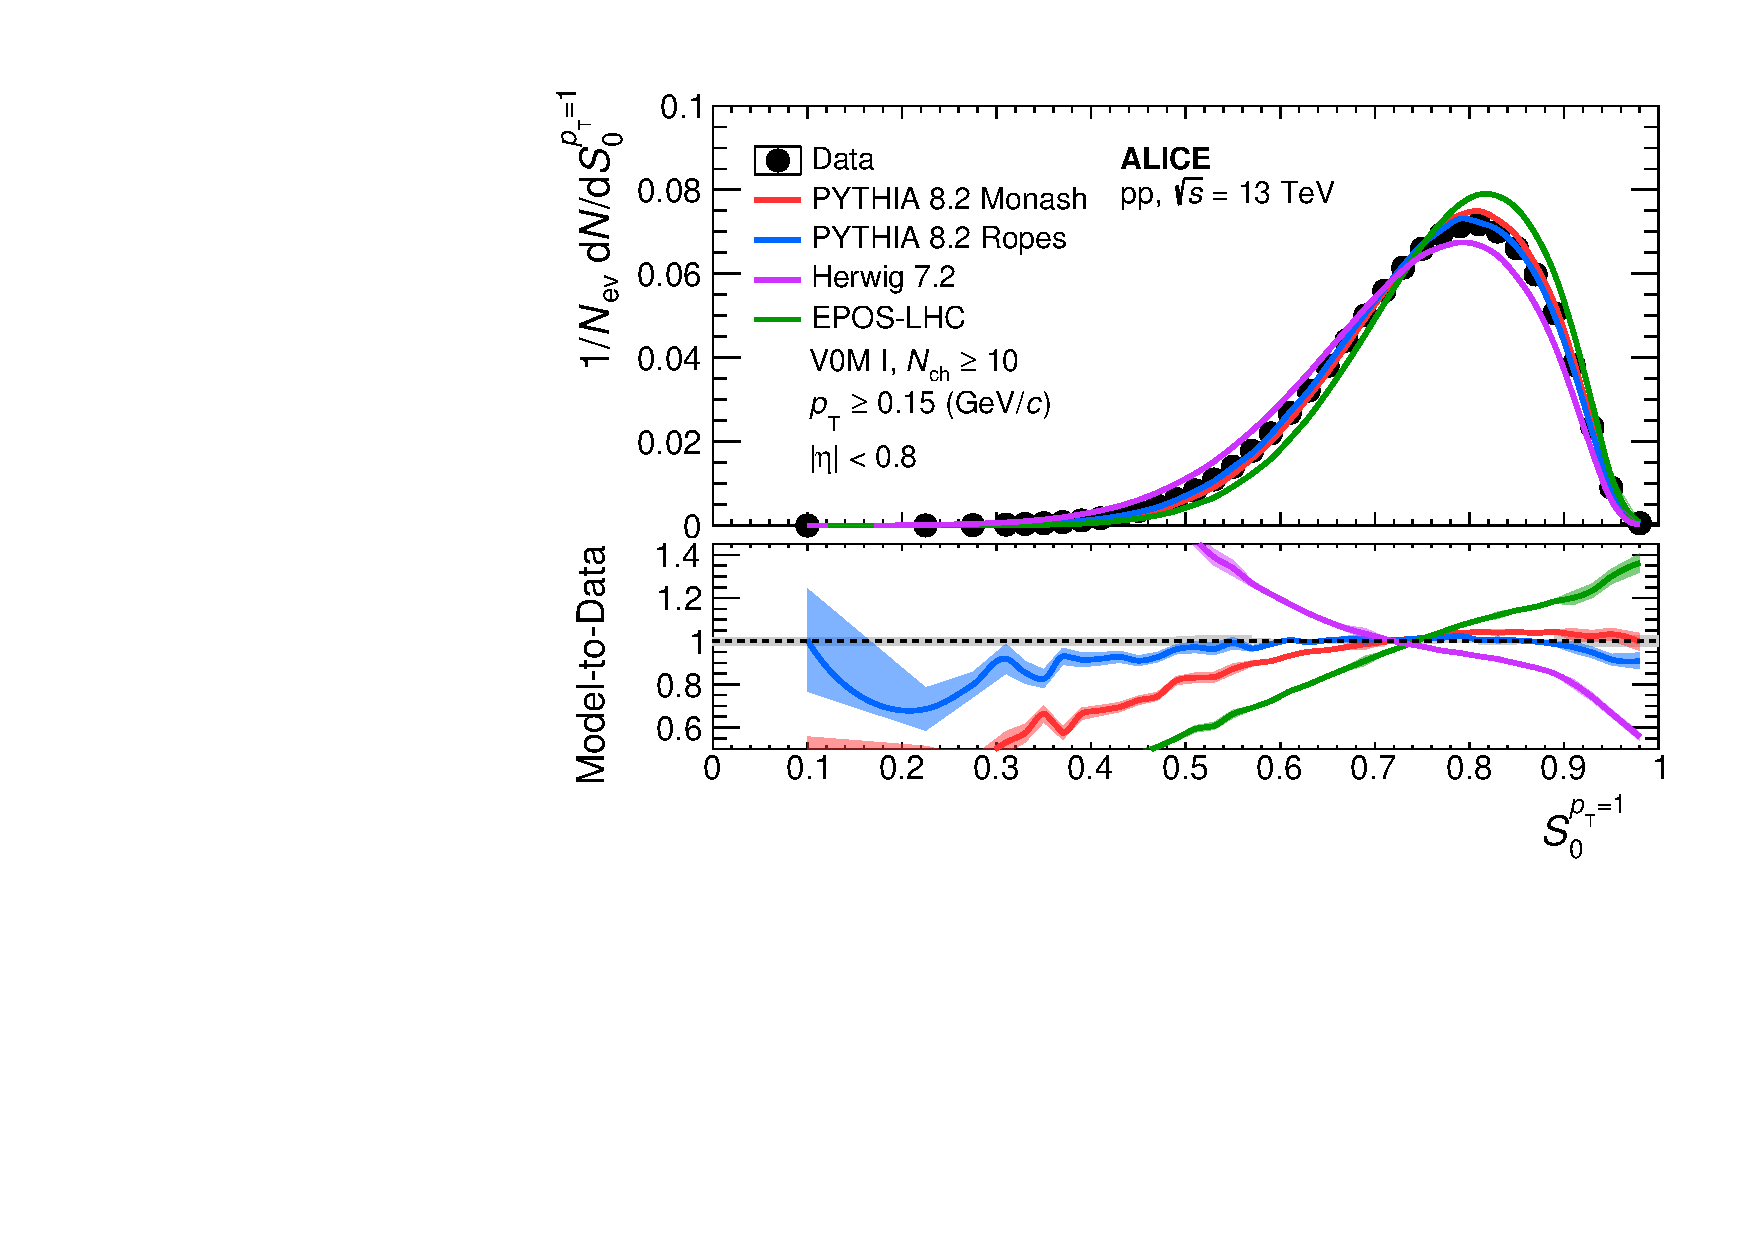
\includegraphics[scale=0.5]{figures/SO_Unfolded_v0m_Perc_I.pdf}
    \caption{Upper panels: The measured and fully corrected \SOPT distributions. Lower panels: Ratio between model calculations and experimental data. These are presented for \tracklet I (top), I-III (middle) and V0M I (bottom). The roman numerals I (I-III) correspond the top 0--1\% (0--10\%) multiplicity for each respective estimator. The curves represent different model predictions, where the shaded area represents the statistical uncertainty of the models. The relative systematic uncertainty is shown as a gray area around unity in the lower panels.}
    \label{Fig:SO}
\end{figure}
\newpage
